\chapter{Desarrollo}

En este capitulo se relata el proceso mes a mes que fue el desarrollo de esta aplicación web. Primero veremos la planificación inicial hablando de los diferentes artefactos que se generaron, posteriormente de como estos evolucionaron y se fueron adaptando y por ultimo del resultado final del desarrollo y lo aprendido en el camino,

\section{Arranque del desarrollo}

El primer artefacto que se genero es el Product Backlog, que recoge todas las funcionalidades deseadas por el cliente, en este caso el equipo médico, en la aplicación en forma de historias de usuario (pequeños fragmentos de texto estructurado que intentan clarificar al máximo las mismas). Este se compone de una tabla con tres columnas; la primera de ellas recoge el grupo en el que se engloba la historia de usuario y su ID, la segunda una descripción corta de la misma y la ultima los criterios del comportamiento que debe tener la funcionalidad en los diversos escenarios posibles.
\newline

La generación de este artefacto fue compleja pues los médicos tenían muy claras dos o tres funcionalidades que supondrán el núcleo de la aplicación como veremos posteriormente, pero del resto de la aplicación o no tenían ninguna petición o no había una opinión firme sobre ellas. Por ellos muchas de las funcionalidades de mediana o baja importancia fueron propuestas por el equipo de desarrollo o el director del TFG y el equipo médico se mostró mas que contento de acogerlas prácticamente todas. A continuación se relatara y explicara cada sección de dicho Product Backlog y las modificaciones que sufrió, el documento completo en pdf para su cómoda lectura va adjunto a esta memoria.
\newpage

El núcleo del que hablábamos anteriormente, y por tanto lo primero a remarcar en nuestro Product Backlog, se compone de estas tres funcionalidades:
\newline

 \begin{figure}[h]
    \centering
     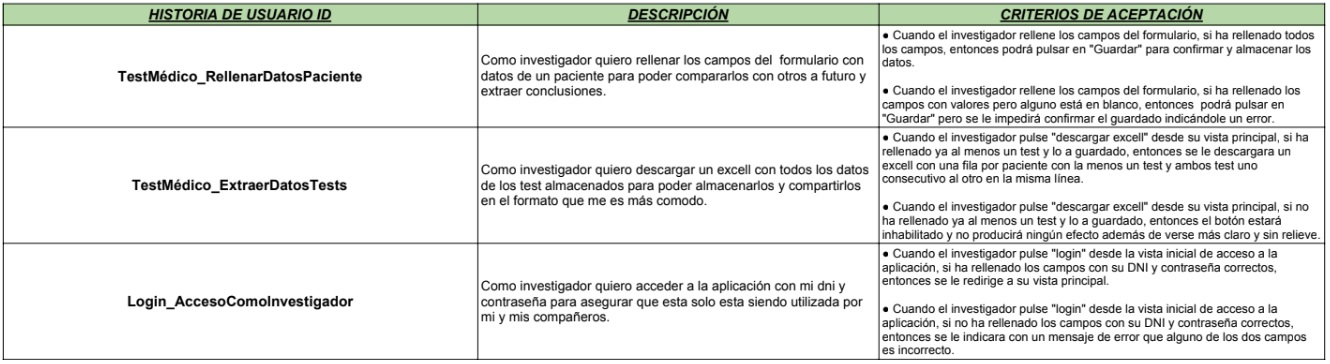
\includegraphics[width=1\textwidth]{images/historiasUsuario-1.jpg}
    \caption{Historias de usuario de mayor importancia, Walking Skeleton de la aplicación.}
\end{figure}


Como se puede apreciar en las historias de usuario lo principal era tener unos test donde rellenar los datos de los pacientes de forma cómoda, que estos datos pudieran luego ser extraídos en un excel y que el acceso a la aplicación fuese privado a los miembros del equipo médico. Las dos primeras suponen la entrada y salida más básica de datos que permitiría al equipo médico extraer sus conclusiones y la tercera, a pesar de ser solo el login podría decirse, el acceso a la aplicación, es también de gran importancia. Uno de los requisitos principales del estudio es el control de la procedencia y gestión de los datos. Únicamente pacientes que se hayan ofrecido voluntariamente vía formulario pueden tener sus datos representados y solo los miembros oficiales del estudio pueden tener acceso a ellos. Esto se consigue mediante un login cerrado que no permite ningún tipo de registro desde el exterior y la creación de todos los perfiles de investigador manualmente por el administrador.
\newline

El siguiente bloque de funcionalidades complementa las tres primeras que en el primer prototipo emplearían perfiles introducidos a mano en la base de datos para probarse:
\newline

 \begin{figure}[h]
    \centering
     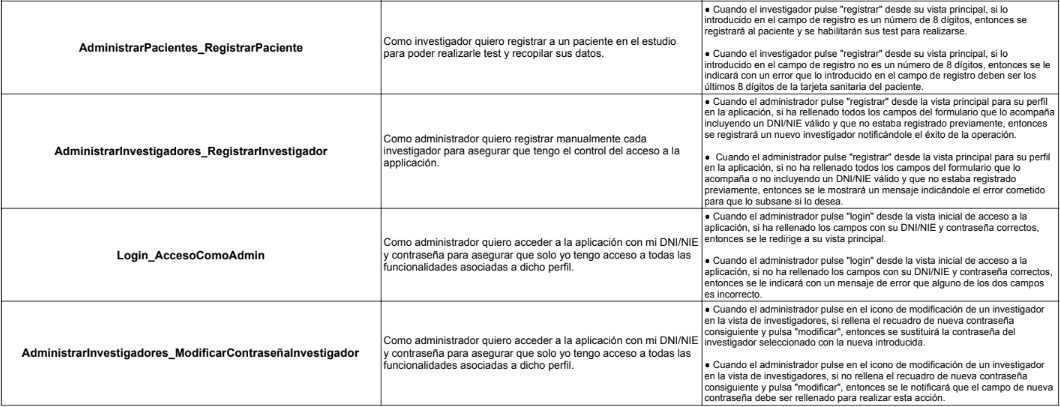
\includegraphics[width=1\textwidth]{images/historiasUsuario-2.jpg}
    \caption{Historias de usuario sobre la inclusión del perfil de administrador y los diversos registros.}
\end{figure}


En este bloque se recogían los registros tanto de pacientes como investigadores así como el perfil de administrador y una funcionalidad que quizá sorprenda encontrarse tan pronto en la escala de prioridades, la modificación de contraseñas. Aparentemente por lo explicado de parte del equipo médico es un problema usual la perdida de contraseña o el filtrado de las mismas por las condiciones de su ambiente de trabajo, y tener un acceso cómodo a su modificación es de gran importancia para ellos. Los desarrolladores lo veían mas como algo secundario pero en este artefacto manda el cliente y así es como se recogió.
\newpage

Las funcionalidades que prosiguieron en la escala de valor para el cliente fueron las siguientes:
\newline

 \begin{figure}[h]
    \centering
     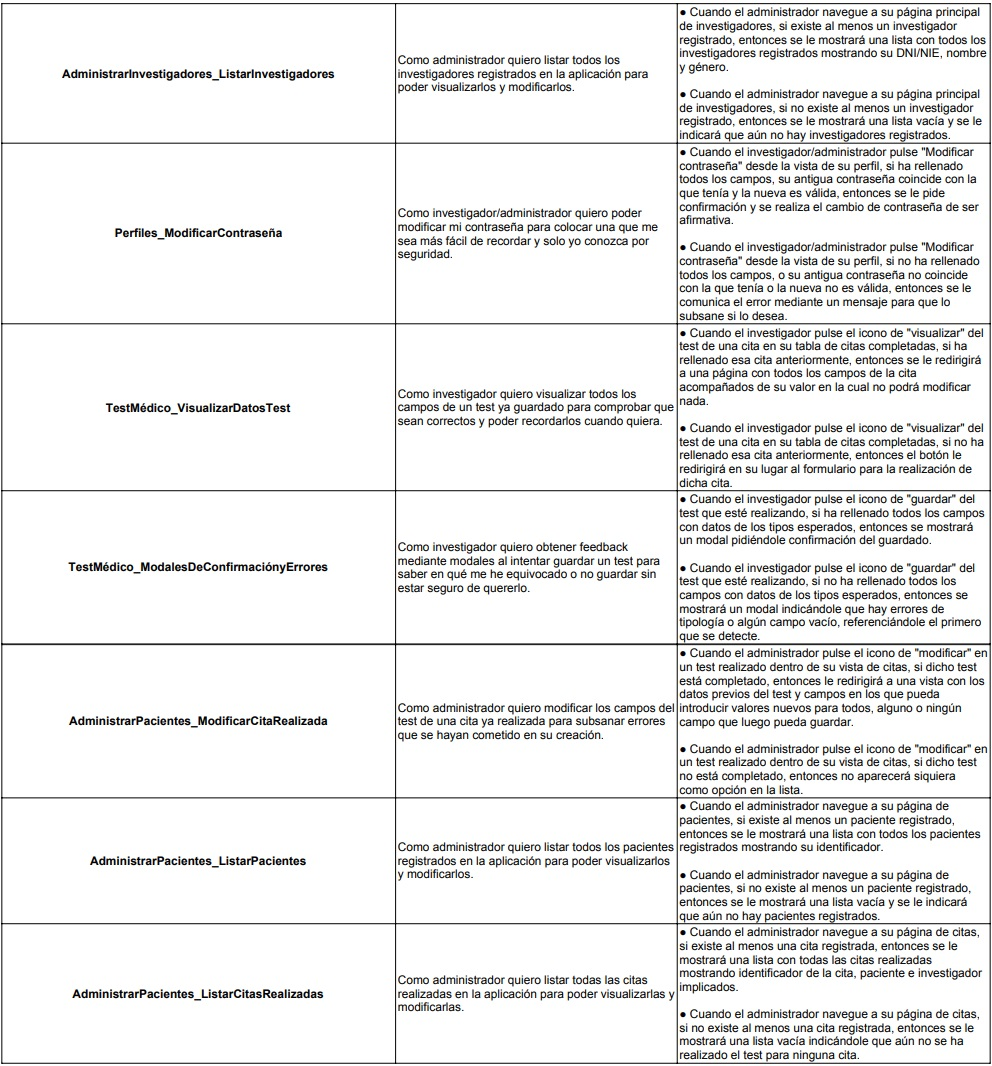
\includegraphics[width=1\textwidth]{images/historiasUsuario-3.jpg}
    \caption{Historias de usuario sobre listado de usuarios y diversas modificaciones.}
\end{figure}


Estas funcionalidades se componen de dos tablas que listen de forma limpia tanto investigadores para el perfil de administrador como pacientes para el de investigador. La funcionalidad de modificar contraseña de nuevo aparece, pero esta vez es para que cada investigador pueda cambiar su propia clave. Esta funcionalidad es principalmente para que el administrador pueda crear sus perfiles con contraseñas que ellos mismos puedan modificar al obtener las cuentas a algo fácil de recordar para ellos mismos. Además se añade la posibilidad de visualizar es una plantilla los datos de un test realizado, ahorrando tener que extraer el excel y consultarlo cada vez cuando solo se quiere revisar el test de una cita en concreto. Se añaden modales para indicar errores y confirmación en los test, importante ya que estos no pueden ser modificados una vez guardados a no ser que lo haga el administrador manualmente. Esta posibilidad de modificar una cita por el administrador es la ultima funcionalidad no comentada de este bloque junto con su listar particular para facilitar el trabajo de este.
\newpage

El penúltimo bloque de funcionalidades que se extrajo al principio del desarrollo empieza a corresponder ya a elementos de gestión necesarios pero no prioritarios que en su mayoría fueron propuestos por el equipo de desarrollo como posibles añadidos prácticos:
\newline

 \begin{figure}[h]
    \centering
     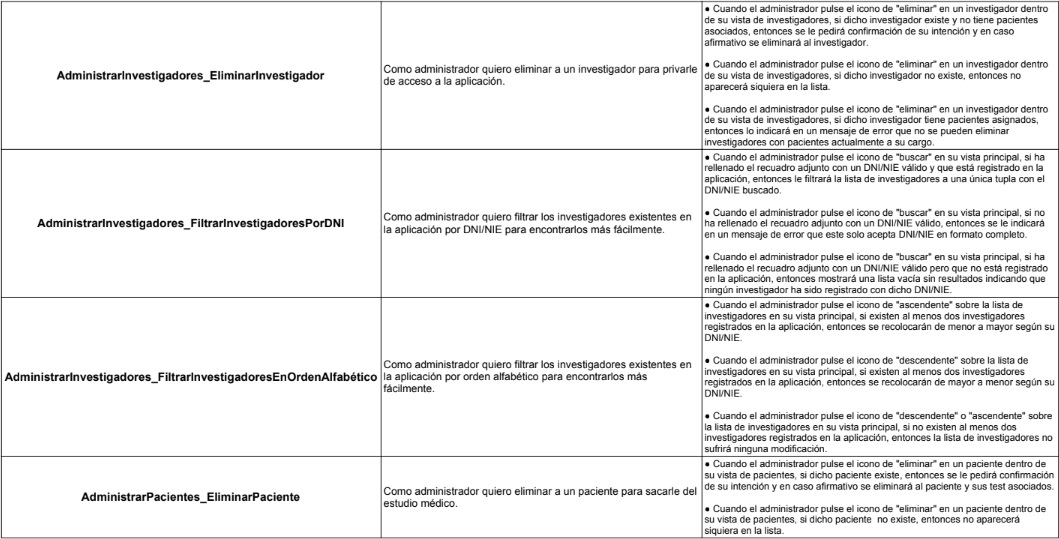
\includegraphics[width=1\textwidth]{images/historiasUsuario-4.jpg}
    \caption{Historias de usuario sobre eliminación de perfiles y agilidad en las búsquedas.}
\end{figure}

Como se puede observar este bloque recogía principalmente la eliminación de perfiles, necesaria si algún paciente o investigador salia del proyecto. Esta funcionalidad aunque simple realmente no se añadió a este artefacto en un primer momento porque generaba dudas por la naturaleza del estudio. Los datos extraídos de la aplicación, para ser validos, deben ser privados, de distintos periodos temporales y completos. La eliminación en este caso de un paciente podía dejar datos incompletos o la de un investigador pacientes con citas a medio completar y cualquiera de estos escenarios invalidaría el estudio. Por ello en primera instancia incluso se pensó en no permitir ningún tipo de eliminación, pero tras debatir con el equipo médico este mismo aseguro que las eliminaciones serian pocas o prácticamente nulas y solo se usarían para subsanar erratas a la hora de crear perfiles nuevos sin afectar los datos. Tras ello se decidió añadirlas no sin delimitar claramente en sus criterios de aceptación las condiciones para poder realizar las eliminaciones.
\newline

La otra funcionalidad que apareció fueron los filtrados, los cuales habían sido implementados en otras aplicaciones por el equipo de desarrollo así que no suponían un gran esfuerzo y podían ser moderadamente útiles. Los médicos no se mostraron entusiastas con la idea pues apenas habría 15 investigadores pero ciertamente era una funcionalidad que podrían usar eventualmente así que se decidió añadirla.
\newpage

El ultimo grupo de funcionalidades que cerraba este artefacto eran las menos prioritarias. Entre ellas un filtrado también para pacientes, la muestra de datos para cada investigador en su propio perfil para los olvidadizos y la inclusión de estadísticas. Esta ultima funcionalidad lamentablemente nunca pudo llevarse al desarrollo pues se prefirió cerrar la aplicación para poder tenerla funcionando y ajustarla a las necesidades del equipo médico a embarcarse en esta funcionalidad que nunca despertó mucho interés en el equipo:
\newline

 \begin{figure}[h]
    \centering
     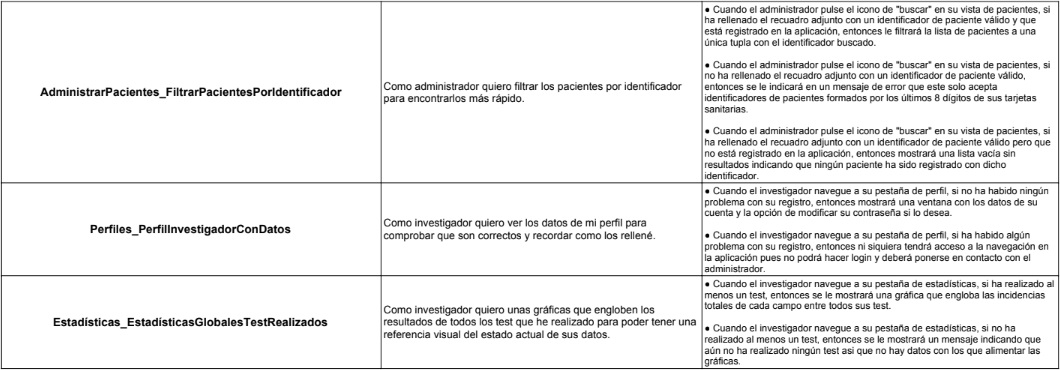
\includegraphics[width=1\textwidth]{images/historiasUsuario-5.jpg}
    \caption{Historias de usuario sobre filtrado de pacientes, perfiles de investigador y estadísticas.}
\end{figure}

Estas fueron todas las funcionalidades añadidas al Product Backlog al principio del desarrollo. Junto a este artefacto se creo también un User Story Map, que permite visualizar mejor todas las historias comentadas anteriormente y además marca un flujo de uso de las mismas de izquierda a derecha y secciona las funcionalidades en las releases mensuales en las que esperábamos tenerlas:
\newline

 \begin{figure}[h]
    \centering
     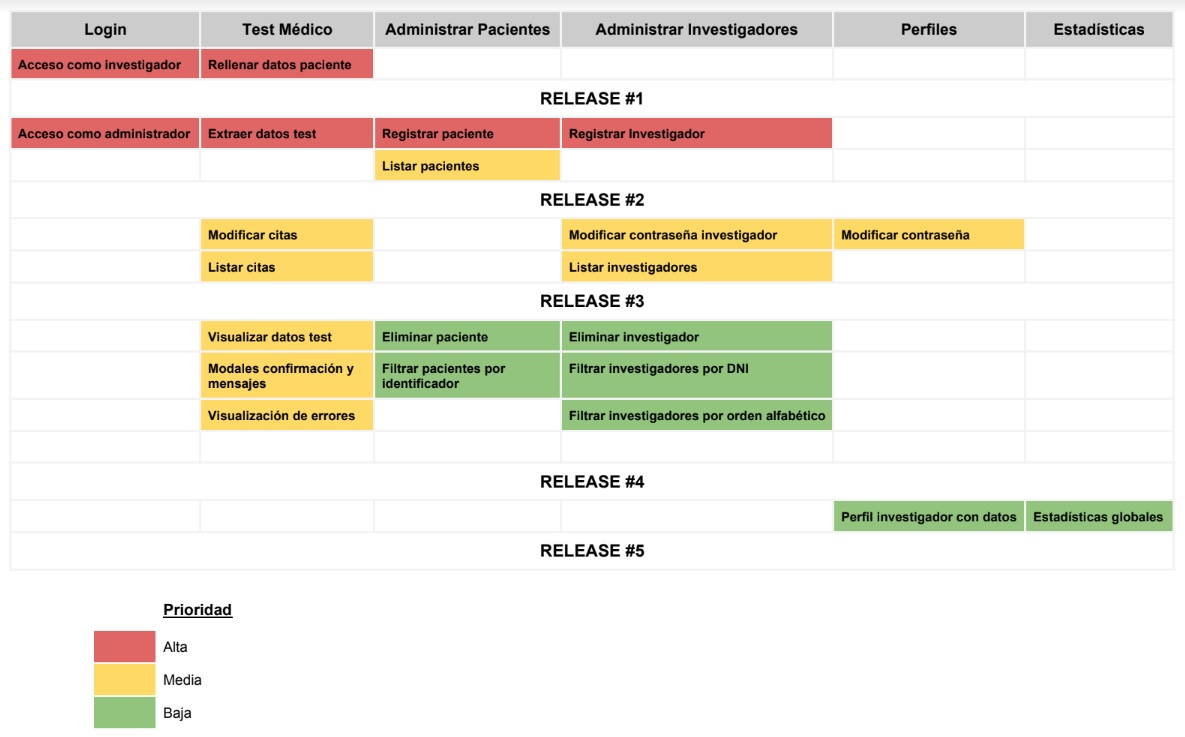
\includegraphics[width=1\textwidth]{images/userStoryMap.jpg}
    \caption{Mapa de historias de usuario.}
\end{figure}
\newpage

\section{Desarrollo durante los sprints}

Con nuestros artefactos listos y la primera reunión fijada para principios de Octubre comenzó nuestro primer sprint en Septiembre. Nuestro objetivo como se puede apreciar en el User Story Map anterior era el acceso a la aplicación como investigador y la posibilidad de rellenar test de pacientes. La idea era empezar con el modelo de datos de los test y de paso pensar en su extracción y después hacer el login, pero faltaban detalles sobre la estructura y limitaciones de los test así que intercambiamos el orden a la espera de información mas precisa. Visto lo cual comenzamos con el acceso a la aplicación.
\newline

A pesar de haber estado durante el mes de agosto viendo tutoriales y trasteando con las tecnologías al ponernos de verdad sobre el proyecto vimos lo verdes que estábamos. Eduardo por suerte en el trabajo que había comenzado ese mismo verano había tocado parte de las herramientas aunque no fuese en profundidad, pero Sergio no había oído casi hablar de herramientas como Angular o Spring Boot hasta hace un par de semanas. El primer mes se nos escapo de las manos prácticamente en configuración del software necesario y de los proyectos tanto en front como back, en la conexión de todo el sistema y el diseño de la simple pagina de login. Para cuando llego Octubre el consumo de tareas iba mucho mas lento de lo esperado y la primera reunión prácticamente solo sirvió para cerrar el diseño de la aplicación en lineas generales, la paleta de colores,el tipo de letra, el espaciado y tamaño, etc. Este retraso en las tareas y desajuste del orden de desarrollo se mantendría lamentablemente para el siguiente sprint aunque se iría ajustando en los siguientes. A continuación se recoge una captura del login, el cual inicialmente tenia una imagen distinta de fondo pero con la misma temática de tener al equipo médico en su ambiente de trabajo, los mismo colores claros entre blanco y azul y la misma letras negra grande.
\newline

 \begin{figure}[h]
    \centering
     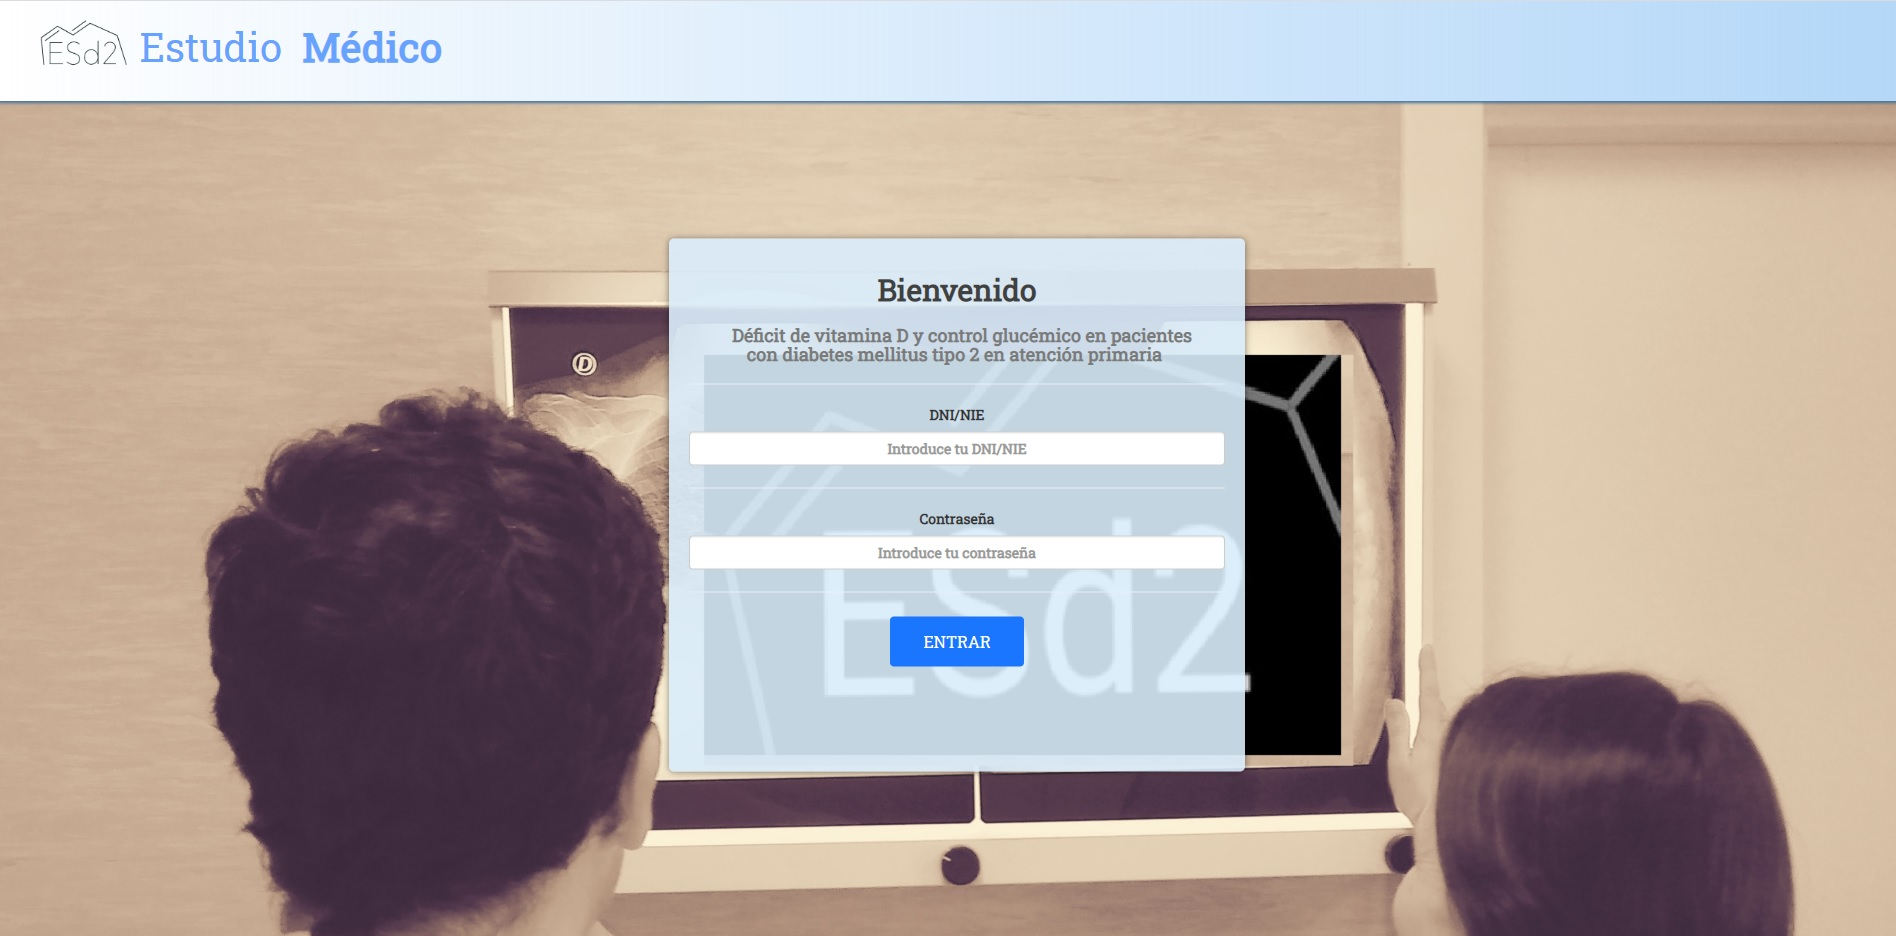
\includegraphics[width=1\textwidth]{images/login.jpg}
    \caption{Captura del login de la aplicación.}
\end{figure}
\newpage